
\documentclass[12pt]{article}
\usepackage{scrextend}
\usepackage[utf8]{inputenc}
\usepackage[polish]{babel}
\usepackage[T1]{fontenc}%polskie znaki
\usepackage[utf8]{inputenc}%polskie znaki
\usepackage{geometry}
\usepackage{float}
\usepackage{enumitem}
\usepackage{hyperref}
\usepackage{graphicx}
\usepackage{tabulary}
\usepackage{etoc}
\usepackage[normalem]{ulem} 
\usepackage{tikz}
\usepackage[bf]{caption}
\usepackage{amsmath}
\usepackage{placeins}

\renewcommand{\baselinestretch}{1.5}

\usepackage{listings}
\usepackage{xcolor}
\usepackage[
    backend=bibtex,
    style=numeric
  ]{biblatex} 

\definecolor{codegreen}{rgb}{0,0.6,0}
\definecolor{codegray}{rgb}{0.5,0.5,0.5}
\definecolor{codepurple}{rgb}{0.58,0,0.82}
\definecolor{backcolour}{rgb}{0.95,0.95,0.92}
 
\lstdefinestyle{mystyle}{
    backgroundcolor=\color{backcolour},   
    commentstyle=\color{codegreen},
    keywordstyle=\color{magenta},
    numberstyle=\tiny\color{codegray},
    stringstyle=\color{codepurple},
    basicstyle=\ttfamily\footnotesize,
    breakatwhitespace=false,         
    breaklines=true,                 
    captionpos=b,                    
    keepspaces=true,                 
    numbers=left,                    
    numbersep=5pt,                  
    showspaces=false,                
    showstringspaces=false,
    showtabs=false,                  
    tabsize=2
}
\renewcommand{\lstlistlistingname}{Spis listingów}\lstset{style=mystyle}

\graphicspath{ {img/} }
\newgeometry{lmargin=2.0cm, rmargin=2.0cm, tmargin=2.0cm, bmargin=2.0cm}
\clubpenalty=9996
\widowpenalty=9999
\brokenpenalty=4991
\predisplaypenalty=10000
\postdisplaypenalty=1549
\displaywidowpenalty=1602

\title{ 
    \vspace*{50mm}
    \textsc{
        \textbf{Rozpoznawanie i przetwarzanie obrazów}\\
        \large Śledzenie stanu stołu bilardowego 
    }
} 
\author{
Damian Koper,  241292\\
Mateusz Gurski, 242089
}

\date{\today}
\bibliography{literature}
\begin{document}

\maketitle

\newpage
\setcounter{tocdepth}{2}
\localtableofcontents
\listoffigures
\lstlistoflistings
\vfill
Repozytorium projektu: \url{https://github.com/damiankoper/ripo}
\newpage

\section{Cel projektu}
Celem projektu było stworzenie systemu umożliwiającego śledzenie stanu stołu podczas gry w bilard. Stan stołu obejmuje pozycję i numer bil obecnych na stole, jak i tych znajdujących się w łuzach. Obejmuje on również pozycje kija gracza.

\subsection{Cele dodatkowe}
Dodatkowym celem było rozpoznanie gracza aktualnie wykonującego ruch oraz zliczanie punktów i sygnalizowanie błędów i fauli.

\section{Stół bilardowy}

Kluczowym elementem projektu jest stół bilardowy. Na etapie projektowania systemu przyjęto następujące założenia dotyczące kamery i stołu:

\begin{enumerate}[noitemsep]
    \item Kamera jest umieszczona nad stołem, prostopadle do płaszczyzny stołu.
    \item Stół musi w całości zawierać się w kadrze zgodnie z orientacją kadru. Nie ma znaczenia jednak przesunięcie i obrót obrazu ($\pm45^\circ$).
    \item Stół musi być dobrze i jednolicie oświetlony.
    \item Przed rozpoczęciem działania systemu, po zmianie pozycji kamery, system musi wykonać proces inicjalizacji, który wymaga usunięcia wszystkich elementów ruchomych ze stołu.
\end{enumerate}

Ze względu na sytuację epidemiczną na terenie Polski w czasie prowadzenia prac nad projektem, nie było możliwości uzyskania dostępu do żadnego stołu, przeprowadzania i nagrania rozgrywki. Posiłkowano się nagraniami rozgrywek dostępnymi w serwisie YouTube z ustawieniami kamery spełniającymi wymagania\cite{youtube}.

\section{Przepływ danych i architektura}

Stworzony system składa się z dwóch głównych komponentów:
\begin{itemize}[noitemsep]
    \item VideoProcessor
    \item PoolVD
\end{itemize}

Komponent \textit{VideoProcessor} zajmuje się przetwarzaniem wideo i komunikacją z komponentem \textit{PoolVD}. Pozyskuje on obraz dostarczony poprzez strumieniem używającym protokołu UDP. Nie użyto tutaj protokołu TCP, ponieważ analiza stołu powinna odbywać się w czasie rzeczywistym i rozwiązanie to wprowadziłoby dodatkowy element synchronizacji, który mógłby mieć wpływ na dostarczany obraz.

Źródłem obrazu może być klip wideo wysyłany z użyciem narzędzie \textit{ffmpeg}, albo obraz na żywo z kamery RaspberryPI. Oba te rozwiązania zostały przetestowane. Wykorzystanie strumienia sieciowego jako źródła obrazu jest rozwiązaniem uniwersalnym, ponieważ oferuje stabilny interfejs po stronie komponentu \textit{VideoProcessor}.

Komponent \textit{VideoProcessor} jest równocześnie serwerem obsługującym połączenia zgodne z protokołem WebSocket. Umożliwia to na szybkie dostarczanie danych wyjściowych do dowolnej liczby klientów. Umożliwia to również na opartą na zdarzeniach komunikację pomiędzy klientami wyświetlającymi dane, omówioną w dalszej części sprawozdania. Protokół WebSocket, w przeciwieństwie do HTTP do dwukierunkowej komunikacji wykorzystuje zawsze jeden strumień.

Przepływ danych od materiału wideo do użytkownika zobrazowane zostało na diagramie z rysunku \ref{dataflow}.


\begin{figure}[!htb]
    \centering
    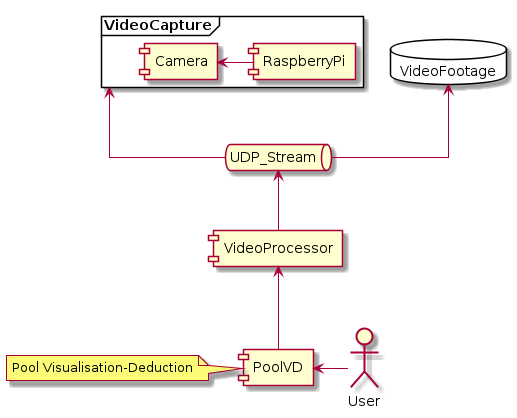
\includegraphics[width=10cm]{./diagrams/out/data_flow.png}
    \caption{Przepływ danych.}
    \label{dataflow}
\end{figure}

\subsection{Architektura}

Detekcja, klasyfikacja, wyświetlania i dedukcja są złożonymi procesami używającymi wiele zasobów sprzętowych. Jednym z filarów sprawnego działania systemu jest sprawny przepływ danych i wielokrotne używanie produktów pośrednich tego przetwarzania. Aby uzyskać płynność przetwarzanego obrazu i optymalne wykorzystanie zasobów wykorzystano podejście wielowątkowe połączone z asynchronicznością.

\subsection{Komponent VideoProcessor}

\begin{figure}[!htb]
    \centering
    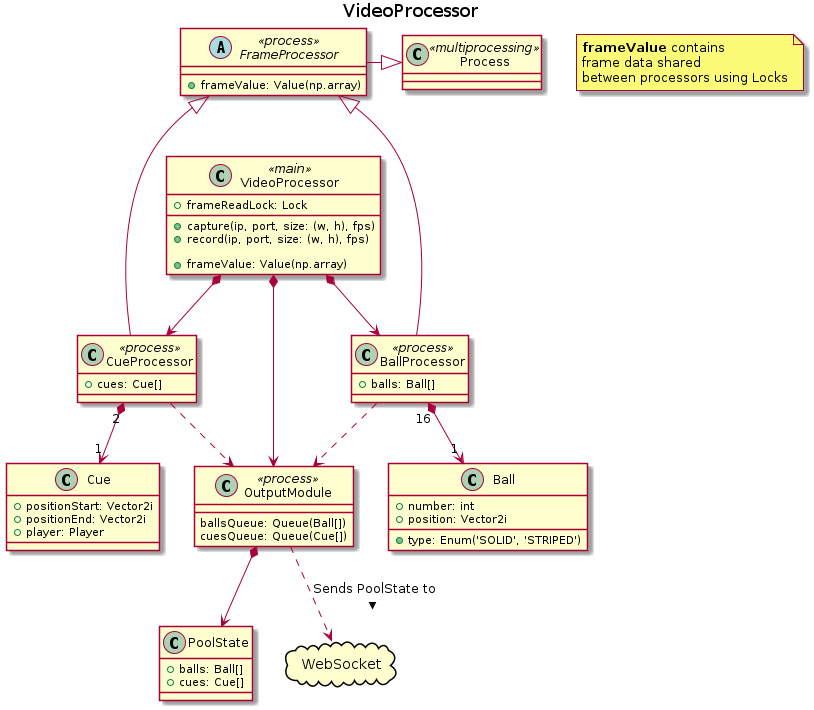
\includegraphics[width=14cm]{./diagrams/out/video_processor_cd.png}
    \caption{Diagram klas komponentu VideoProcessor.}
    \label{vp_cd}
\end{figure}

Punktem wejścia programu jest moduł \lstinline{main}. Przyjmuje on argumenty określające jego działanie - parametry strumienia wejściowego oraz tryb pracy. Może on zostać uruchomiony w trybie domyślnej analizy obrazu lub w celu jego nagrania. Dalszy opis tyczy się trybu analizy obrazu.

Działanie przetwarzania klatki bazuje na działaniu trzech głównych klas - procesów systemowych, nazwanych procesorami. Każdy z nich posiada swój rozbudowany obiekt konfiguracji. Ogólną strukturę klas komponentu przedstawia diagram na rysunku~\ref{vp_cd}.

\begin{enumerate}
    \item \textbf{VideoProcessor}. Nazwa taka sama jak nazwa całego komponentu. Klasa odpowiedzialna za odebranie klatki i oddanie sterowania do klasy \lstinline{InitialFrameProcessing} w celu wykonania procesu inicjalizacji i wstępnego przetworzenia klatki. Po wstępnym przetworzeniu umieszcza ona produkty tego przetwarzania klatki w zmiennych współdzielonych pomiędzy innymi klasami - procesorami.
    \item \textbf{BallProcessor}. Klasa odpowiedzialna za detekcję i klasyfikację bil. W celu klasyfikacji wykrytych bil klasa ta przekazuje sterowanie do klasy \lstinline{Classification}.
    \item \textbf{CueProcessor}. Klasa odpowiedzialna za detekcję kija. %TODO MAti jak się się zmieniło to dopisz tu ogólnie
\end{enumerate}

Procesy \textbf{BallProcessor} i \textbf{CueProcessor} przed rozpoczęciem przetwarzania oczekują na klatkę, jeśli nie jest ona dostępna. Dzięki funkcjonowaniu zmiennych współdzielonych, w których przekazywane są klatki przez \textbf{VideoProcessor}, oba procesory w momencie rozpoczęcia przetwarzania pobierają zawsze aktualne dane. Pozwala to na przetwarzanie niezależnie od wydajności algorytmów w poszczególnych klasach.

Po zakończeniu przetwarzania każdej klatki \textbf{BallProcessor} i \textbf{CueProcessor} wysyłają wynik swoich działań w postaci obiektów \lstinline{Ball} lub \lstinline{Cue} do kolejek modułu OutputModule.

\subsubsection{OutputModule}

OutputModule jest osobnym procesem, który obsługuje trzy procedury:
\begin{enumerate} [noitemsep]
    \item Serwer komunikacji zewnętrznej - \lstinline{WebSocketServer}.
    \item Obserwator kolejki wykrytych bili.
    \item Obserwator kolejki wykrytych kijów.
\end{enumerate}

\begin{figure}[!htb]
    \centering
    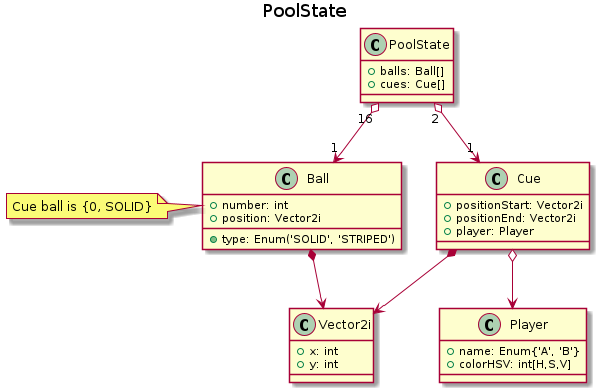
\includegraphics[width=9cm]{./diagrams/out/pull_state_cd.png}
    \caption{Struktura PoolState.}
    \label{poolstate}
\end{figure}

Moduł zawiera również ostatni aktualny wykryty stan stołu. Strukturę te prezentuje diagram na rysunku \ref{poolstate}.
Obserwatory obserwujące kolejkę, po umieszczeniu w nich danych przez moduły \textbf{BallProcessor} i \textbf{CueProcessor} aktualizują obiekt \lstinline{PoolState} i wymuszają wysłanie stanu stołu do klientów przez serwer.

Protokół WebSocket umożliwia komunikację full-duplex w dowolny sposób. W celu ustandaryzowania komunikacji pomiędzy klientami, a serwerem zdecydowano się wybrać zorientowaną zdarzeniowo bibliotekę Socket.IO \cite{socket.io}.

Proces przesyłania stanu stołu do komponentu \textbf{PoolVD} obrazuje diagram na rysunku \ref{pool_state_sd}. Obsługę zdarzenia zmiany opcji czasu trwania okresu inicjalizacji z poziomu interfejsu użytkownika prezentuje diagram na rysunku \ref{pool_vd_events_sd}.

\begin{figure}[!htb]
    \centering
    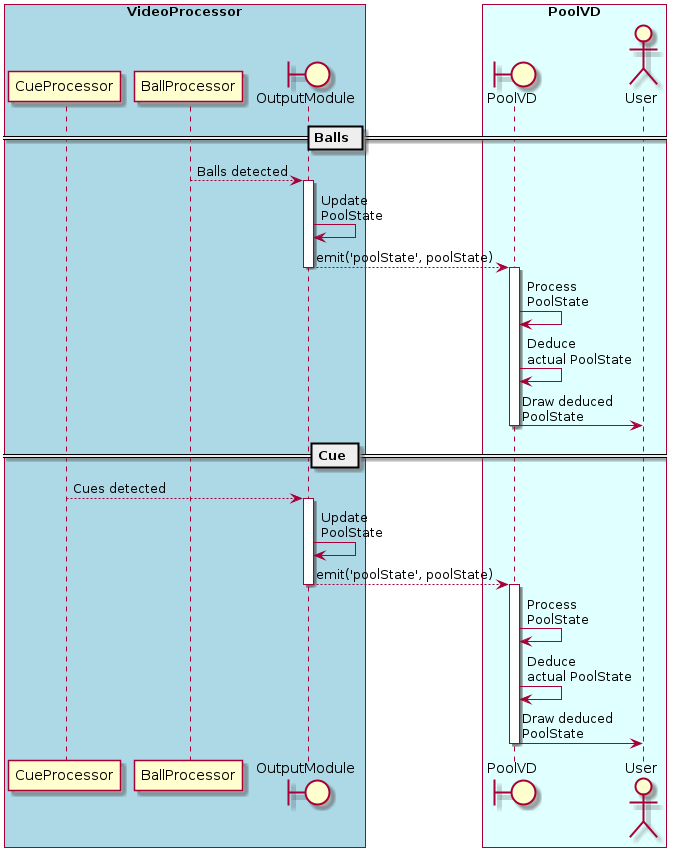
\includegraphics[width=15cm]{./diagrams/out/pool_state_sd.png}
    \caption{Proces przesyłania stanu stołu do komponentu \textbf{PoolVD}.}
    \label{pool_state_sd}
\end{figure}


Każda z klas obsługujących zdarzenia ma dostęp do swojej kolejki, w której \textbf{OutputModule} umieszcza przychodzące obiekty zdarzeń. Klasa obsługuje tylko takie zdarzenia, których obsługa została przewidziana i ignoruje nieznane. Rozwiązanie to pozwala na łatwe rozszerzenie konfiguracji i zachowania każdej z klas bez żadnego wpływu na inne klasy - wystarczy tylko zaimplementować odbiór i obsługę nowego zdarzenia.


\begin{figure}[!htb]
    \centering
    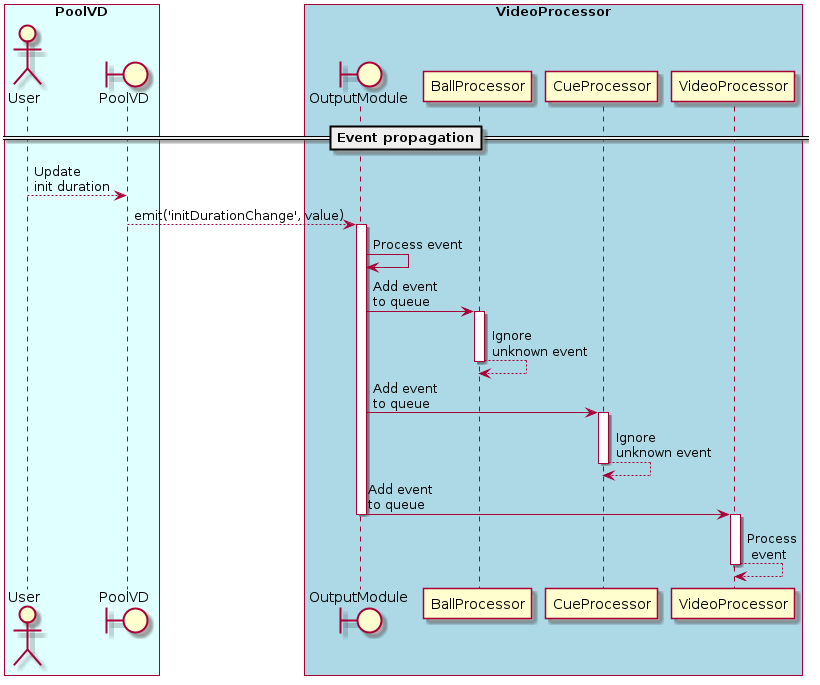
\includegraphics[width=15cm]{./diagrams/out/pool_vd_events_sd.png}
    \caption{Obsługa zdarzenia wywołanego przez \textbf{PoolVD}.}
    \label{pool_vd_events_sd}
\end{figure}

\subsection{Komponent PoolVD}
Komponent PoolVD odpowiada za wyświetlanie otrzymanego stanu stołu, odrzucanie stanów nieprawdopodobnych i śledzenie wpadnięć bili do łuz. Wysyła on również zdarzenia do komponentu \textbf{VideoProcessor}, które aktualizują parametry detekcji i wywołują zdefiniowane akcje.

Komponent tworzy historię stanów stołu. Na tej podstawie wykonuje następujące procedury dla każdej bili:

\begin{enumerate} [noitemsep]
    \item Wyświetlanie ostatniego otrzymanego stanu. Eliminuje to tymczasowe zniknięcia bili spowodowane błędem detekcji, klasyfikacji, albo zasłonięciem bili przez inny obiekt.
    \item Odrzucenie stanów nieprawdopodobnych. Na podstawie stanów poprzednich, przychodzący stan bili może być odrzucony, jeśli bila przemieściła się nienaturalnie szybko w inną część stołu. Odrzuca to pojedyncze błędy klasyfikacji. Heurystyką używaną w tym wnioskowaniu jest prędkość średnia bili uzyskana na podstawie poprzednich stanów.
    \item Wykrycie wpadnięcia bili do łuzy. Bila jest uznana za wpadniętą do łuzy jeśli przez konfigurowalną liczbę stanów była niewykryta, a jej ostatnia znana była pozycją blisko danej łuzy.
\end{enumerate}

Każda z procedur ma konfigurowalną precyzję podaną jako liczbę stanów.

\section{Detekcja i klasyfikacja}

Cały proces detekcji i klasyfikacji rozpoczyna się w \textbf{VideoProcessor} gdzie pozyskiwany jest obraz i wykonywany jest wstępny proces jego przetwarzania. Przetwarzanie obrazu odbywa się z wykorzystaniem biblioteki OpenCV \cite{OpenCV}.

\begin{figure}[!htb]
    \centering
    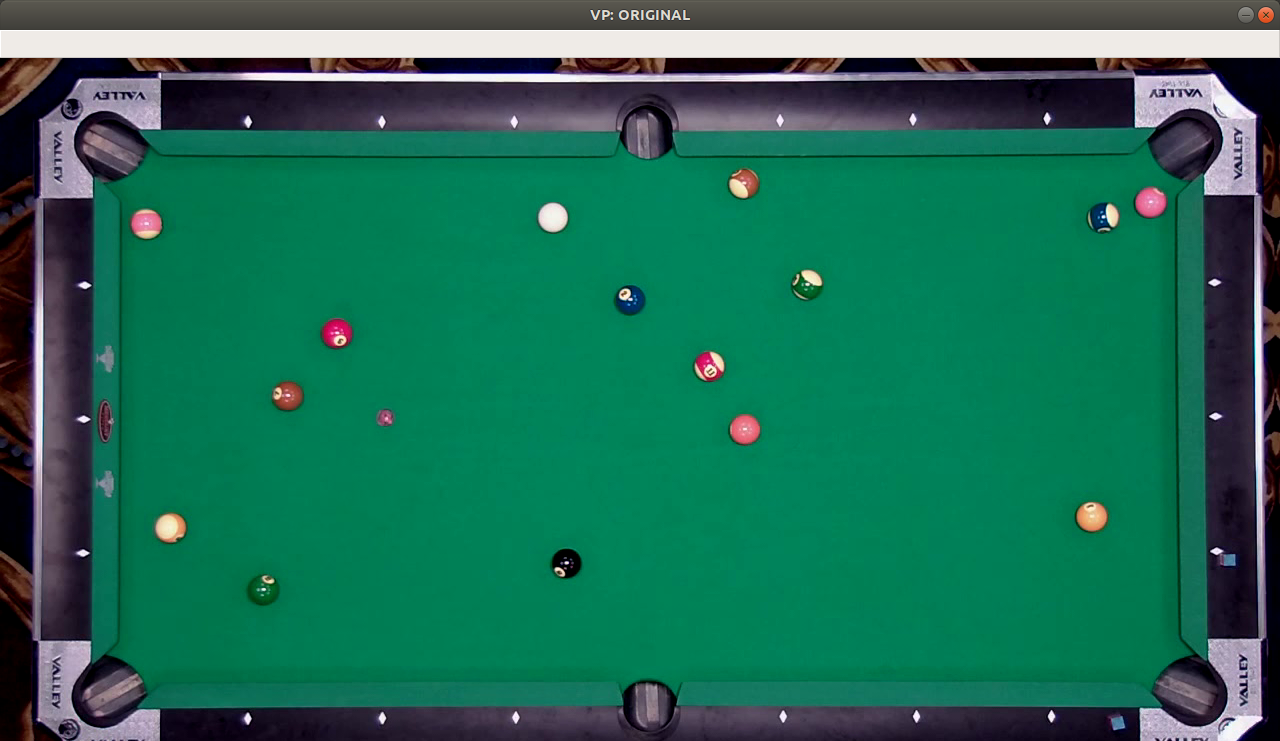
\includegraphics[width=15cm]{./images/obrazki/vp/original.png}
    \caption{Oryginalna klatka pozyskiwana w \textbf{VideoProcessor}.}
    \label{vp_original}
\end{figure}

\subsection{Proces inicjalizacji}

Proces inicjalizacji powinien odbywać się na pustym stole, przed rozpoczęciem gry. Jego głównym celem jest uzyskanie uśrednionej klatki obrazu zawierającej pusty stół, który w kolejnych etapach odejmowany jest od aktualnej klatki obrazu w celu wyizolowania istotnych z punktu widzenia detekcji elementów – bil i kijów. Proces inicjalizacji zwraca obraz tła – uśredniony pusty stół. Ustala również sposób wycinania i obracania kolejnych klatek. Dane potrzebne do dalszego przetwarzania dostępne są już po przeanalizowaniu jednej klatki, jednak dłuższy czas jego trwania pozwala na uzyskanie lepiej uśrednionej klatki i lepszej macierzy transformacji. 
\clearpage

Etapy przetwarzania podczas procesu inicjalizacji to kolejno:
    \begin{enumerate} [noitemsep]
        \item Uśrednianie klatki
        \item Detekcja stołu (na podstawie uśrednionej klatki).
        \item Polepszanie macierzy transformacji (na podstawie uśrednionej klatki).
    \end{enumerate}
    
    Uśredniona klatka konwertowana jest na przestrzeń kolorów HSV (hue, saturation, value), gdzie Hue - reprezentuje typ koloru, Saturation - reprezentuje intensywność koloru a Value - reprezentuje jasność koloru. Ponieważ typ koloru modelowany jest tylko przez kanał Hue, segmentacja części obrazu na podstawie koloru łatwiejsza jest w przestrzeni HSV niż w przestrzeni barw RGB, gdzie kolory kodowane są przy użyciu trzech kanałów.
    Po konwersji uśrednionej klatki na przestrzeń barw HSV, tworzona jest maska, na podstawie dolnej i górnej granicy zakresu wartości pikseli w przestrzeni kolorów HSV. Granice te konfigurowalne są z poziomu interfejsu użytkownika. Uzyskana maska przedstawiona jest na rysunku \ref{pool_table_mask}.

    \begin{figure}[!htb]
        \centering
        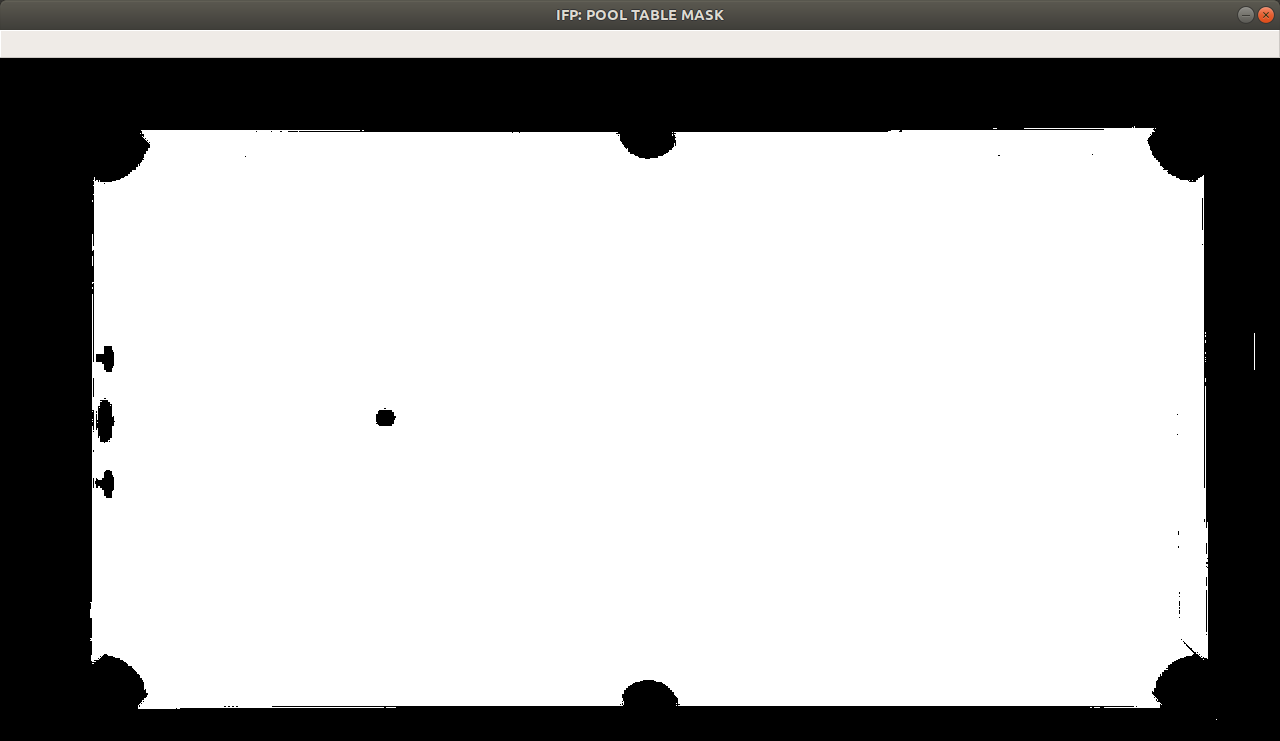
\includegraphics[width=15cm]{./images/obrazki/inicjalizacja/pool_table_mask.png}
        \caption{Uzyskiwana w procesie inicjalizacji maska.}
        \label{pool_table_mask}
    \end{figure}


        Przy użyciu funkcji \textbf{findContours} opisanej na stronie \cite{FindContours} w otrzymanej masce znajdywany jest największy kontur, do którego zostaje dopasowany prostokąt, co przedstawione zostało na rysunku \ref{detected_pool_table}.

    \begin{figure}[!htb]
        \centering
        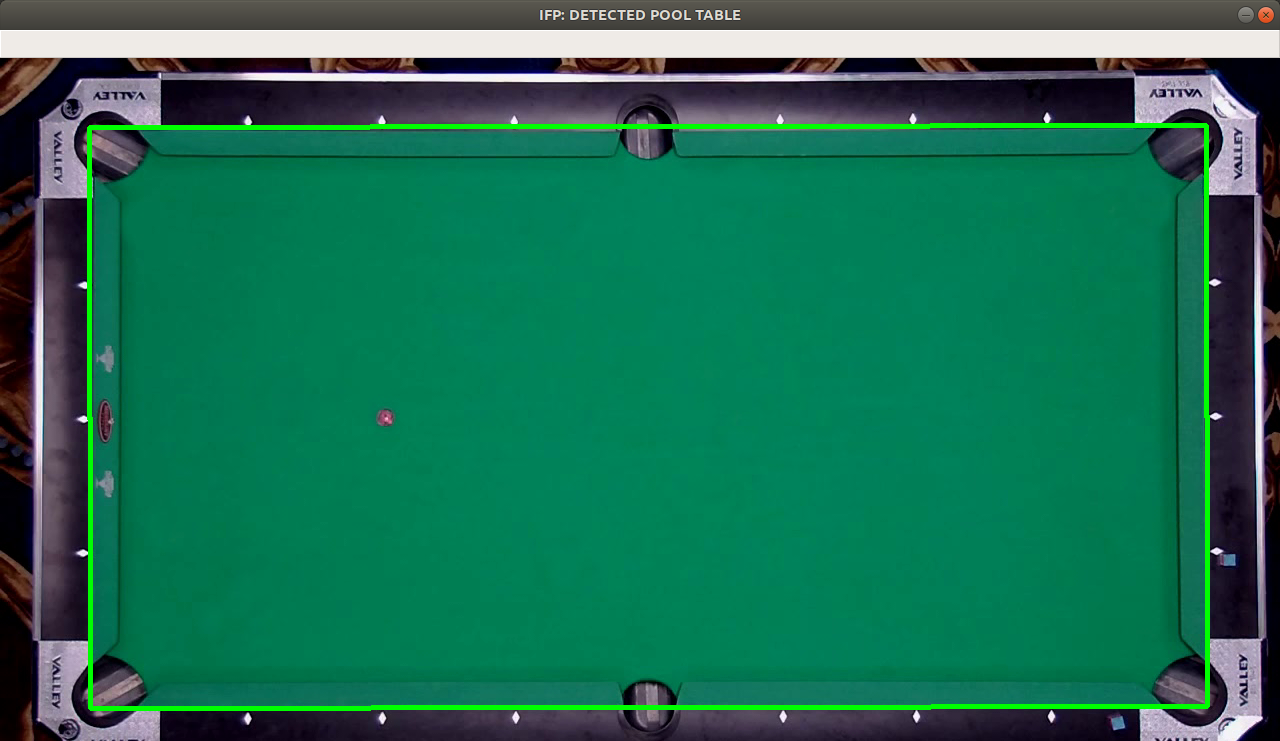
\includegraphics[width=15cm]{./images/obrazki/inicjalizacja/detected_pool_table.png}
        \caption{Wykryty stół.}
        \label{detected_pool_table}
    \end{figure}


    Granice znalezionego prostokąta, a dokładniej 4 pary współrzędnych jego rogów wykorzystywane są do utworzenia macierzy transformacji przy użyciu metody \textbf{getPerspectiveTransform} opisanej na stronie \cite{getPerspectiveTransform}, macierz ta polepszana jest z czasem trwania procesu inicjalizacji ze względu na uśrednianie klatki, które powoduje uzyskiwanie lepszych wartości współrzędnych rogów stołu. Utworzona macierz transformacji pozwala na wykonanie transformacji perspektywicznej w celu uzyskania odpowiednio wyciętego i obróconego stołu wypełniającego całą ramkę. W tym celu wykorzystana została metoda \textbf{warpPerspective} opisana na stronie \cite{warpPerspective}.  


\subsection{Produkty przetwarzania wstępnego}

Produktami przetwarzania wstępnego są klatka uśredniona przedstawiona na rysunku \ref{avg_frame} oraz odpowiednio wycięta aktualna klatka obrazu przedstawiona na rysunku \ref{warped_frame}. Obie te klatki przekazywane są dalej do kolejnych procesorów – \textbf{BallProcessor} i \textbf{CueProcessor}, a \textbf{VideoProcessor} zajmuje się dalej, nie czekając, przetwarzaniem kolejnej klatki obrazu.


\begin{figure}[h]
    \centering
    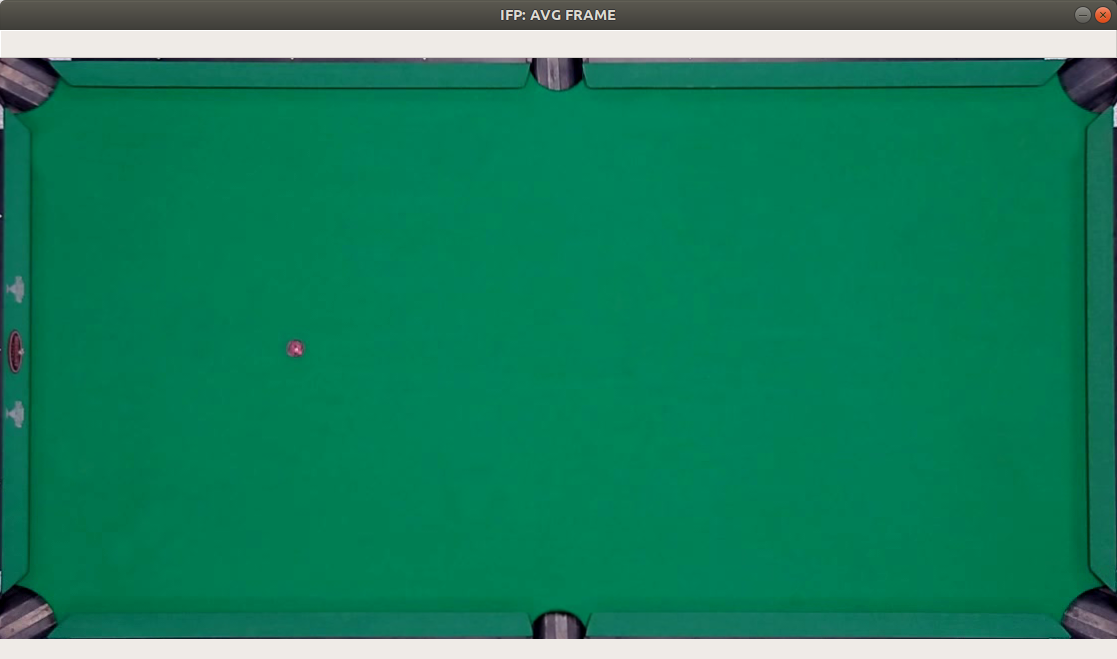
\includegraphics[width=15cm]{./images/obrazki/ifp/avg_frame.png}
    \caption{Uśredniona i wycięta klatka.}
    \label{avg_frame}
\end{figure}

\begin{figure}[h]
    \centering
    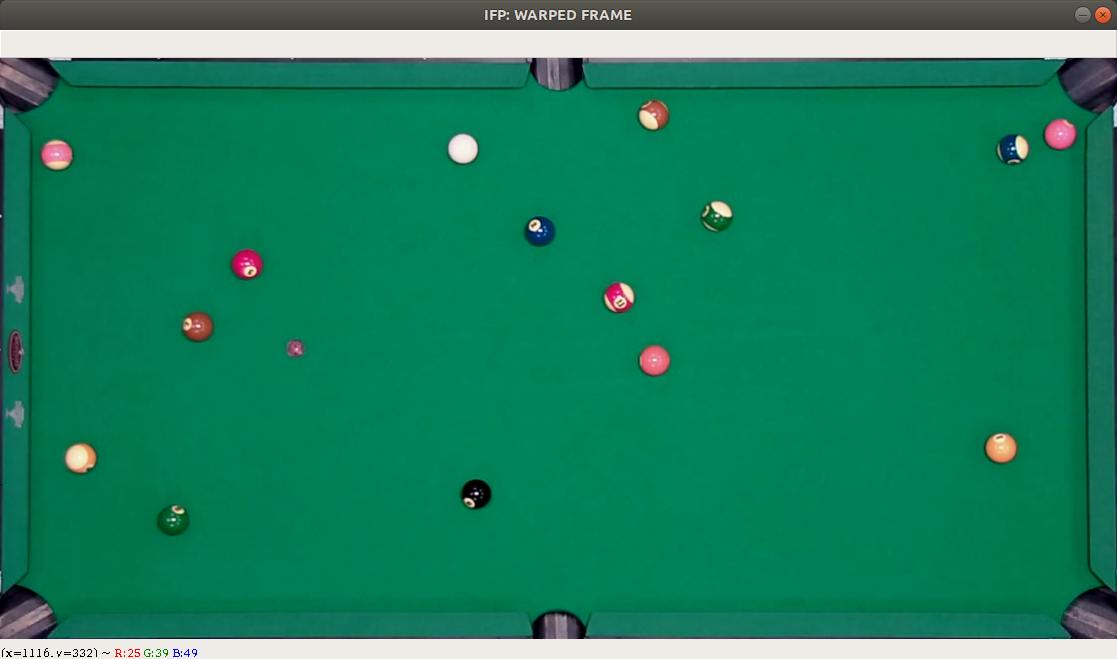
\includegraphics[width=15cm]{./images/obrazki/ifp/warped_frame.png}
    \caption{Odpowiednio wycięta aktualna klatka obrazu.}
    \label{warped_frame}
\end{figure}

\clearpage

\subsection{Bile}

\subsubsection{Detekcja}

    Od odpowiednio wyciętej aktualnej klatki obrazu odejmowane jest tło  oraz wykonywana jest konwersja do skali szarości. Uzyskiwany w ten sposób efekt przedstawiony został na rysunku~\ref{bp_diff}.

    \begin{figure}[h]
        \centering
        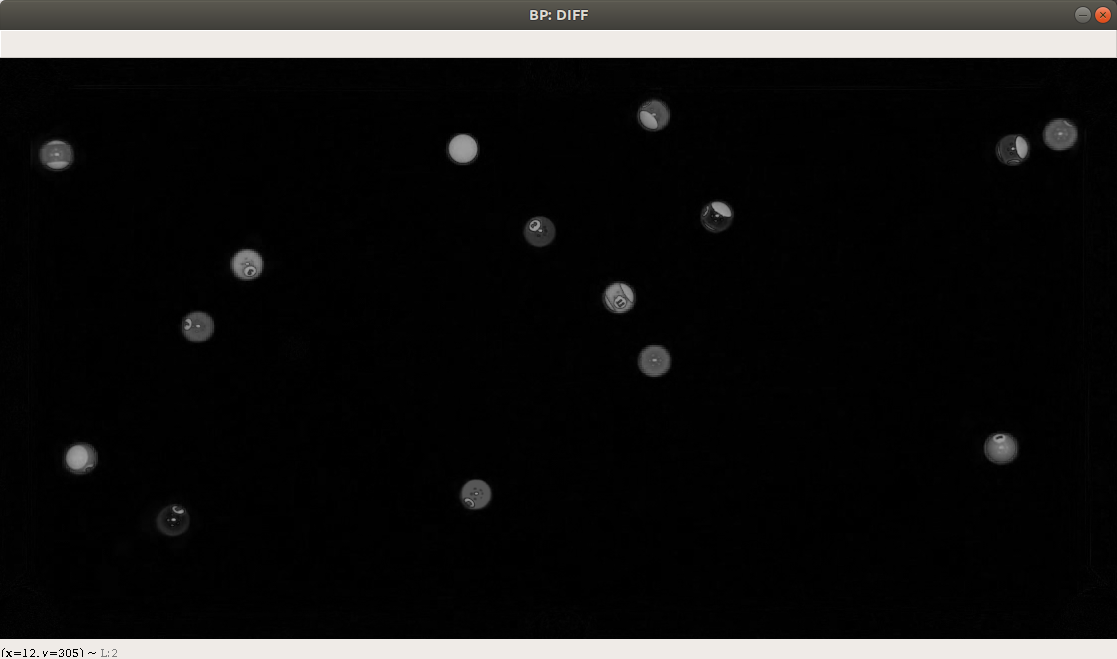
\includegraphics[width=15cm]{./images/obrazki/bp/bp_diff.png}
        \caption{Różnica aktualnej klatki z klatką uśrednioną w skali szarości.}
        \label{bp_diff}
    \end{figure}


    W celu uzyskania maski wykonywane jest progowanie (wartość progowa konfigurowalna jest dynamicznie z poziomu interfejsu użytkownika). W celu uwydatnienia istotnych elementów – w tym przypadku bil, oraz usunięcia szumów, wykonywane są również operacje morfologiczne.
    \vspace{0.5cm}
    
    Przetestowane zostały różne kombinacje i częstotliwości operacji otwarcia, domknięcia oraz samych erozji - które powodują usunięcie tych punktów obrazu o wartości 1, których sąsiedztwo opisane przez podany kernel nie jest w każdym przypadku równe 1 i dylatacji - działającej odwrotnie, wartość piksela zmieniana jest na 1 gdy przynajmniej 1 piksel w sąsiedztwie jest równy 1. Ostatecznie, operacje, które pozwalają uzyskać najlepszy w tym przypadku efekt przy utrzymaniu odpowiedniej wydajności są operacje:

    \begin{enumerate}
        \item otwarcia – erozji, po której następuje dylatacja, która dobrze sprawdza się do usuwania szumów z obrazu.
        \item domknięcia – dylatacji, po której następuje erozja. Przydatna do zapełniania/domykania konturów.
    \end{enumerate}

    Różnice między sprogowanym obrazem przed i po operacjach morfologicznych przedstawione zostały na rysunkach \ref{thresh_before_morph} i \ref{thresh_after_morph}. Opis metody \textbf{morphologyEx}, która została wykorzystana w celu zastosowania opisanych operacji morfologicznych znajduje się na stronie \cite{morphologyEx}.

    \begin{figure}[h]
        \centering
        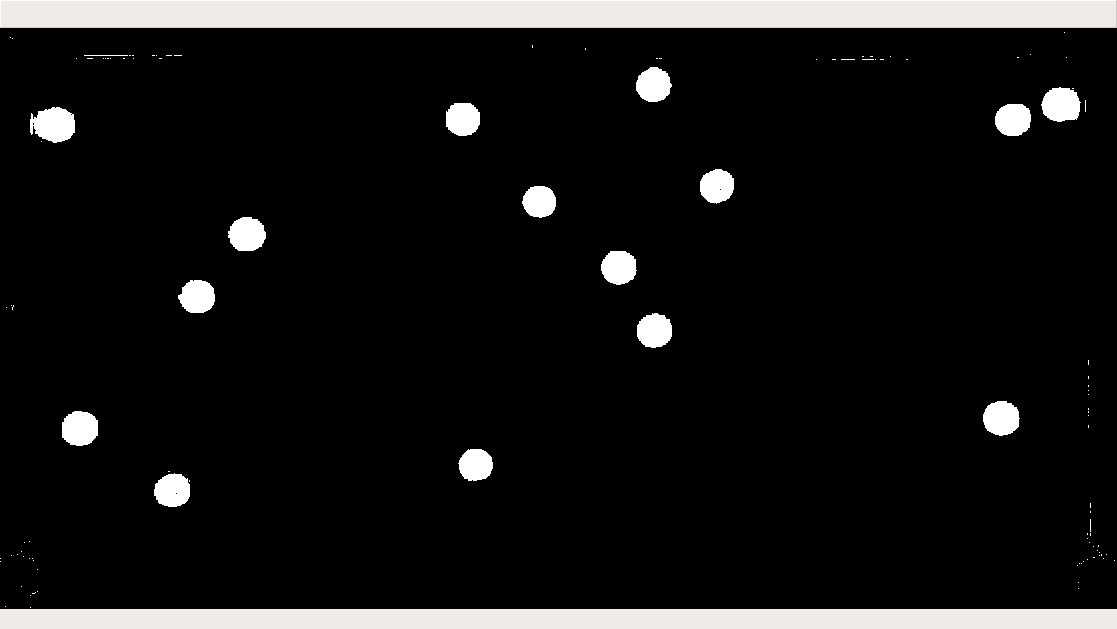
\includegraphics[width=15cm]{./images/obrazki/bp/thresh_before_morph.png}
        \caption{Sprogowany obraz przed przeprowadzeniem operacji morfologicznych.}
        \label{thresh_before_morph}
    \end{figure}

    \begin{figure}[h]
        \centering
        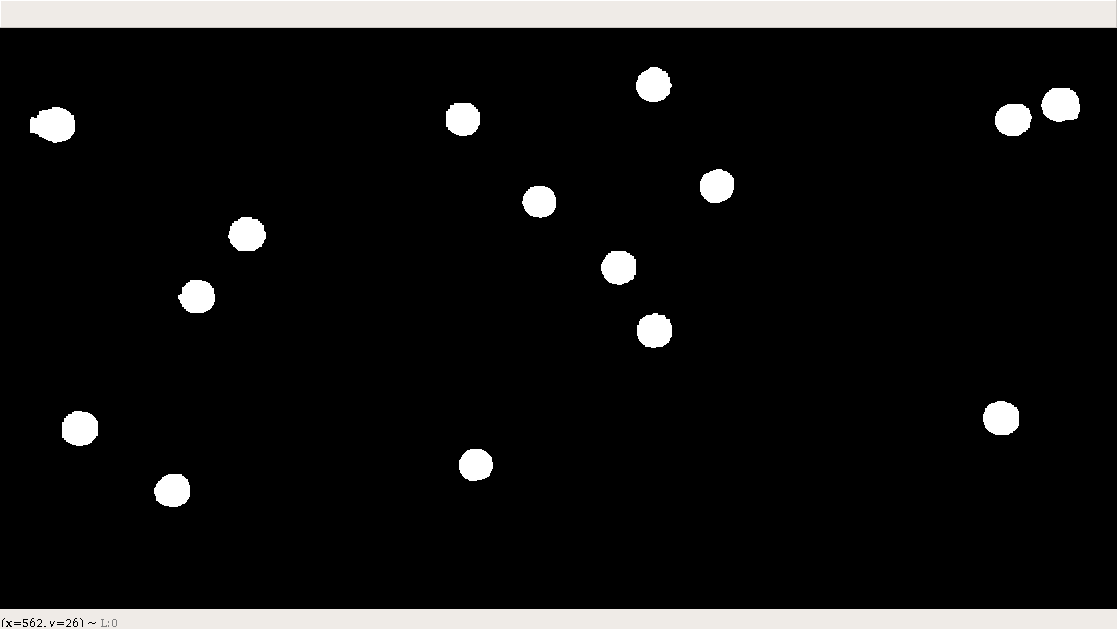
\includegraphics[width=15cm]{./images/obrazki/bp/thresh_contours.png}
        \caption{Sprogowany obraz po przeprowadzeniu operacji morfologicznych.}
        \label{thresh_after_morph}
    \end{figure}
    
    Detekcja bil odbywa się dwuetapowo wykorzystując połączenie dwóch metod – \textbf{FindCountours} \cite{FindContours} oraz \textbf{HoughCircles} \cite{HoughCircles}.

    Pierwszym etapem detekcji jest metoda \textbf{FindContours}, która po odpowiednim dostrojeniu pozwala na stosunkowo szybkie wykrycie konturów bil. Dostrojenie tej metody w przypadku wykrywania bil, polega na sprawdzaniu czy znalezione kontury spełniają warunki kolistego kształtu oraz czy długość ich promienia znajduję się w odpowiednim przedziale. Metoda \textbf{FindContours} okazała się być bardziej wydajna i stabilna jeśli chodzi o wykrywane współrzędne od metody \textbf{HoughCircles}. Doskonale radzi sobie ona jeśli chodzi o wykrywanie bil, które znajdują się daleko od siebie co przedstawiono zostało na rysunku \ref{bp_detected}, nie generuje też ona fałszywych detekcji co ma miejsce w przypadku metody \textbf{HoughCircles}, nie radzi ona sobie jednak w przypadku bil znajdujących się blisko siebie lub blisko gracza – co powoduje sklejenie ich konturów co widać na rysunku \ref{thresh_before_hc} i tym samym uniemożliwia ich wykrycie. Dla takich przypadków powstał drugi etap detekcji, czyli wykorzystanie metody \textbf{HoughCircles}. Znalezione w pierwszym etapie bile zostają zamalowane a maska, która może zawierać niewykryte bile przechodzi dalej, do drugiego etapu, gdzie użycie metody \textbf{HoughCircles} pozwoli wykryć te bile, których nie udało się wykryć w tym etapie.

    \begin{figure}[!htb]
        \centering
        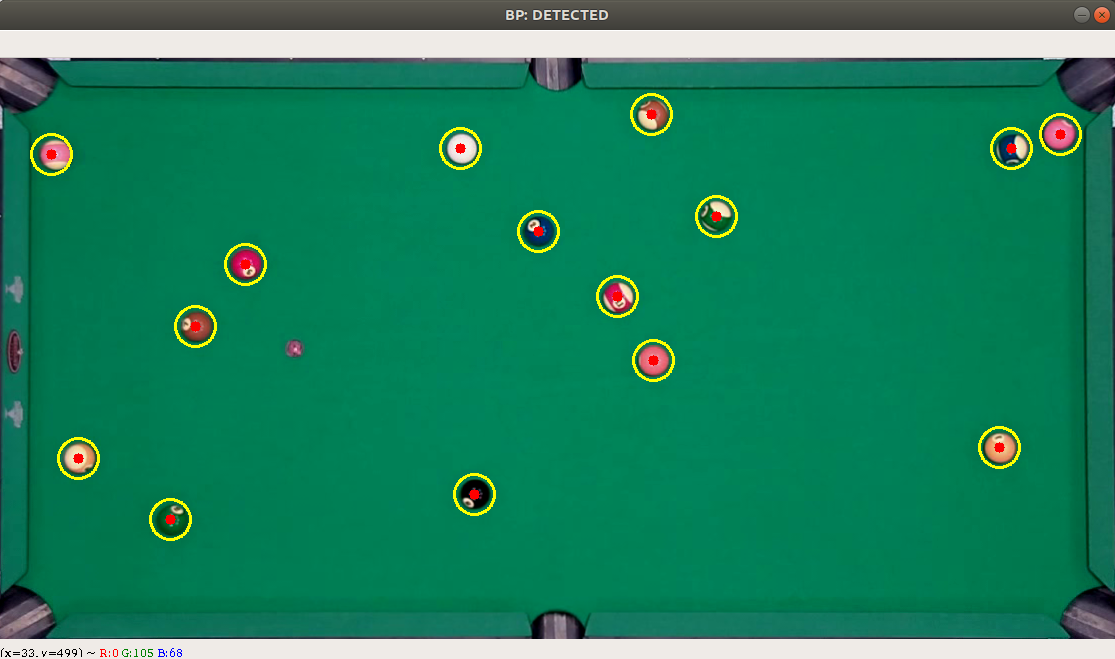
\includegraphics[width=15cm]{./images/obrazki/bp/bp_detected.png}
        \caption{Bile znajdujące się daleko od siebie - znalezione przy użyciu \textbf{FindContours}.}
        \label{bp_detected}
    \end{figure}


    \begin{figure}[!htb]
        \centering
        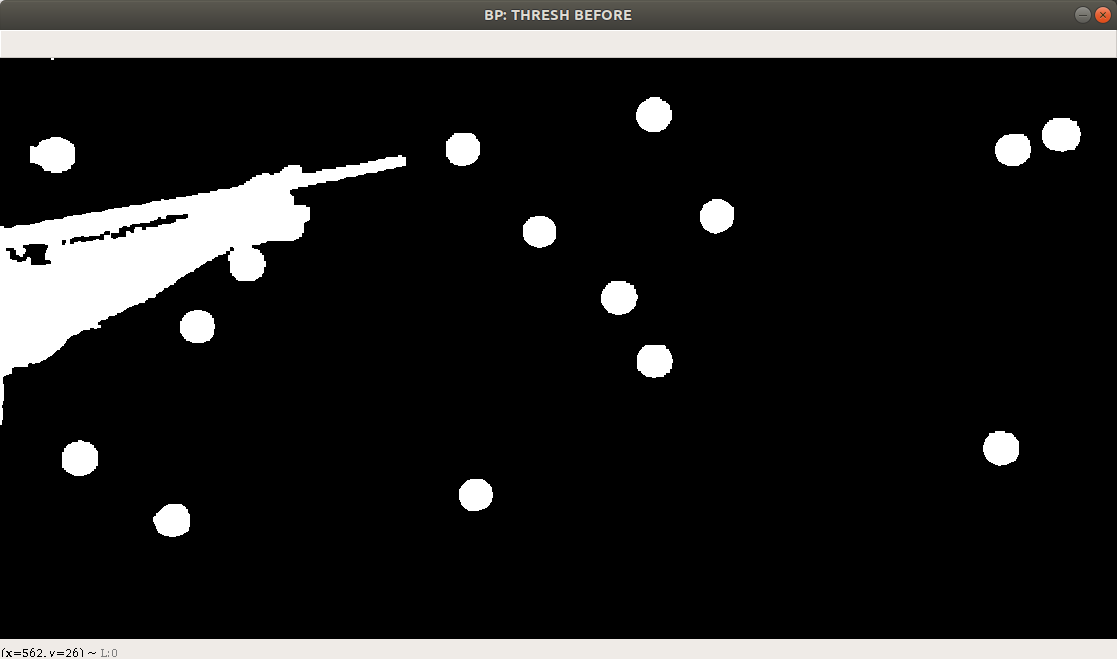
\includegraphics[width=15cm]{./images/obrazki/bp/thresh_before_hc2.png}
        \caption{Sklejenie konturu gracza i bili znajdującej się obok niego.}
        \label{thresh_before_hc}
    \end{figure}

    Drugim etapem detekcji jest metoda \textbf{HoughCircles}, która wykorzystuje modyfikację oryginalej transformacji Hougha (metody wykrywania prostych) pozwalającą na wykrywanie kolistych kształtów. Algorytm \textbf{Circle Hough Transform} opisany jest na stronie \cite{CirclesHoughTransform} a metoda \textbf{HoughCircles} opisana jest na stronie \cite{HoughCircles}. Jest ona mniej wydajna od \textbf{FindContours}, powoduje więcej fałszywych wykryć, a przede wszystkim jest mniej stabilna jeśli chodzi o wykryte współrzędne środków bil, co wyklucza ją jako podstawową i jedyną metodę detekcji. Pozwala ona jednak na detekcję nawet bardzo trudnych do wykrycia bil i bardzo dobrze spełnia się w roli detekcji pomocniczej - tam gdzie \textbf{FindContours} nie da rady. Zmodyfikowana w poprzednim etapie maska poprzez zamalowanie już wykrytych bil przedstawiona na rysunku \ref{thresh_hc} zostaje nałożona na różnicę klatek. Otrzymany w ten sposób obraz przedstawiony na rysunku \ref{masked_hc} przekazywany jest do metody \textbf{HoughCircles}.
  
    \begin{figure}[!htb]
        \centering
        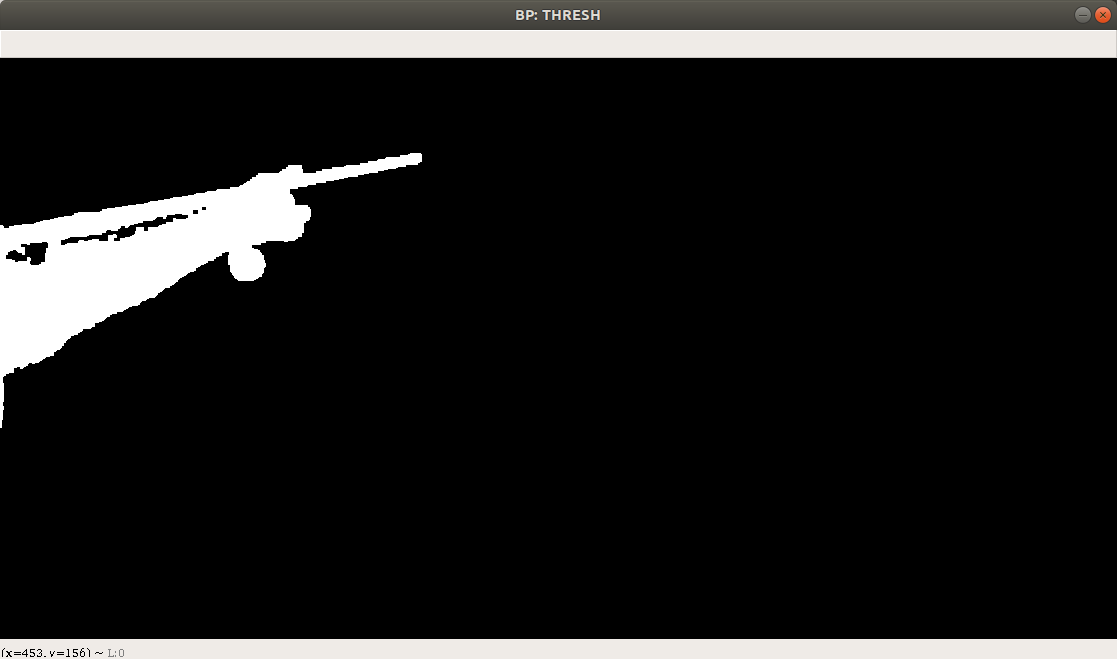
\includegraphics[width=15cm]{./images/obrazki/bp/thresh_hc.png}
        \caption{Uzyskana po pierwszym etapie maska z niewykrytą jedną bilą.}
        \label{thresh_hc}
    \end{figure}

    \begin{figure}[!htb]
        \centering
        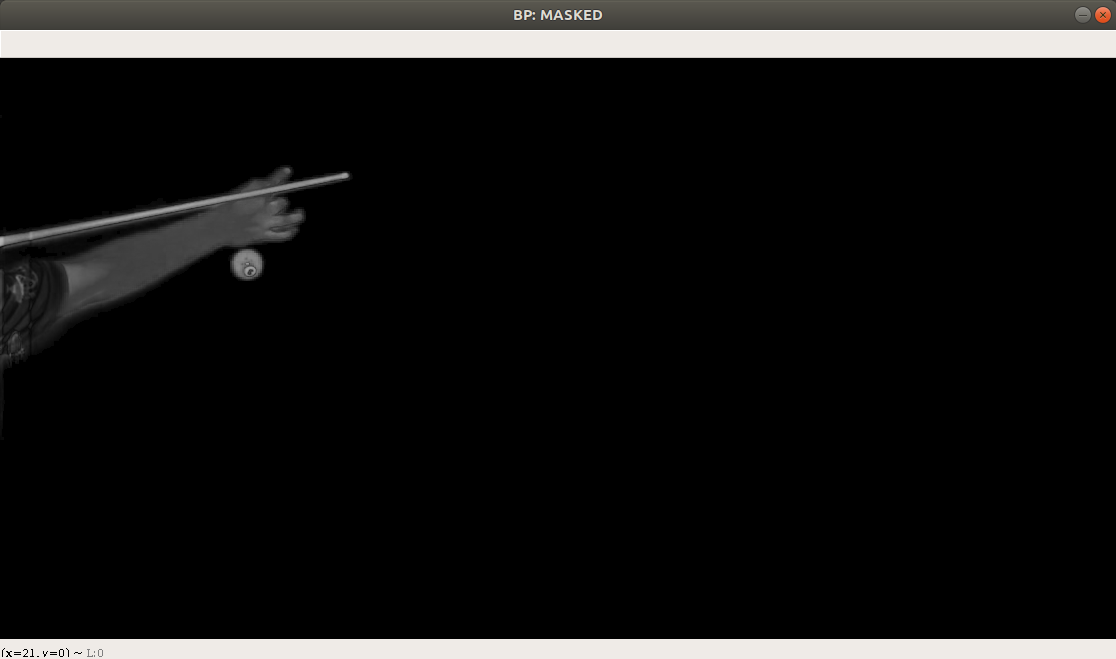
\includegraphics[width=15cm]{./images/obrazki/bp/masked_hc.png}
        \caption{Nałożenie maski na różnice tła i klatki aktualnej.}
        \label{masked_hc}
    \end{figure}

    \begin{figure}[!htb]
        \centering
        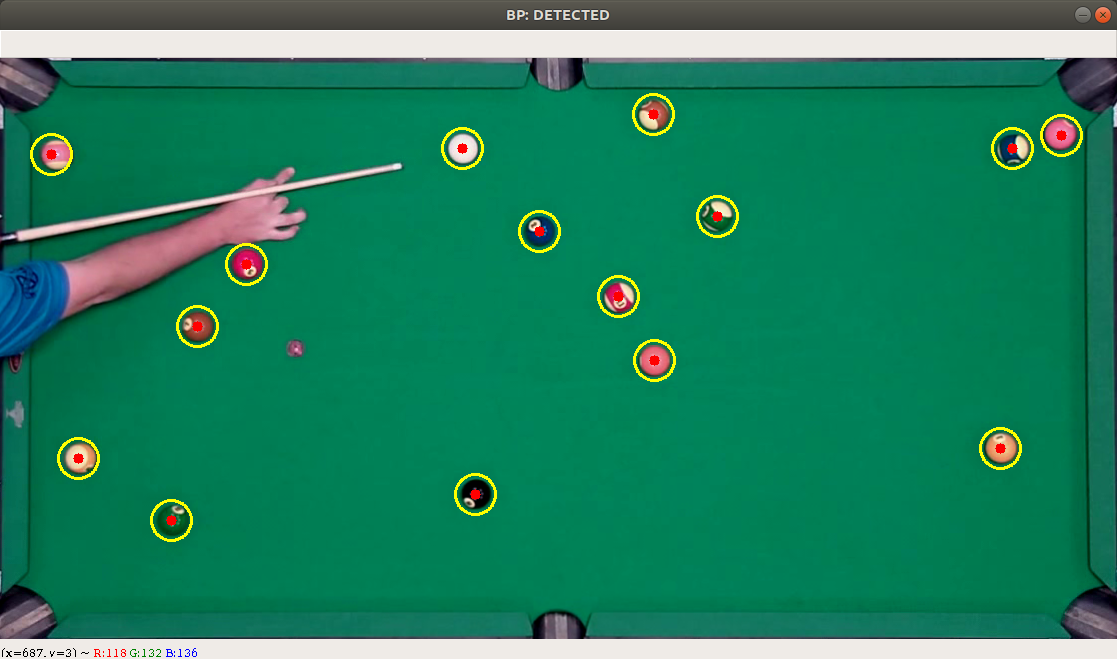
\includegraphics[width=15cm]{./images/obrazki/bp/bp_detected_2.png}
        \caption{Wykryte bile po obu etapach detekcji.}
        \label{bp_detected2}
    \end{figure}

    Ostatecznie otrzymywana jest lista współrzędnych środków wykrytych bil (rysunek \ref{bp_detected2}). Dla każdego z nich wycinany jest obraz bili w rozmiarze 50x50, który klasyfikowany jest przy użyciu konwolucyjnej sieci neuronowej.
 
    \subsubsection{Klasyfikacja}

    
    Do utworzenia sieci neuronowej wykorzystany został framework \textbf{Tensorflow} \cite{TensorFlow} i \textbf{Keras} \cite{keras}. Głównym wyzwaniem było uzyskanie odpowiedniej jakości klasyfikacji przy jednoczesnym utrzymaniu odpowiedniej wydajności.
    Ostateczny model sieci składa się z powtórzonej sekwencji dwóch warstw konwolucyjnych, po których następują warstwa łącząca oraz warstwa dropout. Na końcu do wsparcia ostatecznej klasyfikacji wykorzystywane są dwie klasyczne warstwy gęsto rozłożonych neuronów. 
    
    
    Możliwość uruchomienia aplikacji w trybie, w którym wykrywane bile zapisywane są do pliku pozwoliła na zebranie własnego datasetu – który następnie został ręcznie poetykietowany. Utworzona została również metoda rozszerzania i zapewniania unikalności datasetu - każdy element datasetu mnożony jest 10 krotnie oraz poddawany jest losowym transformacjom – losowe odbicia w pionie i poziomie, przesunięcia, oraz obroty o losowy kąt z ustalonego przedziału. Pozwoliło to na utworzenie datasetu złożonego z \textbf{16.000 unikalnych obrazów bil} oraz \textbf{1.000 obrazów fałszywych – błędów detekcji}.

    \begin{figure}[!htb]
       \centering
       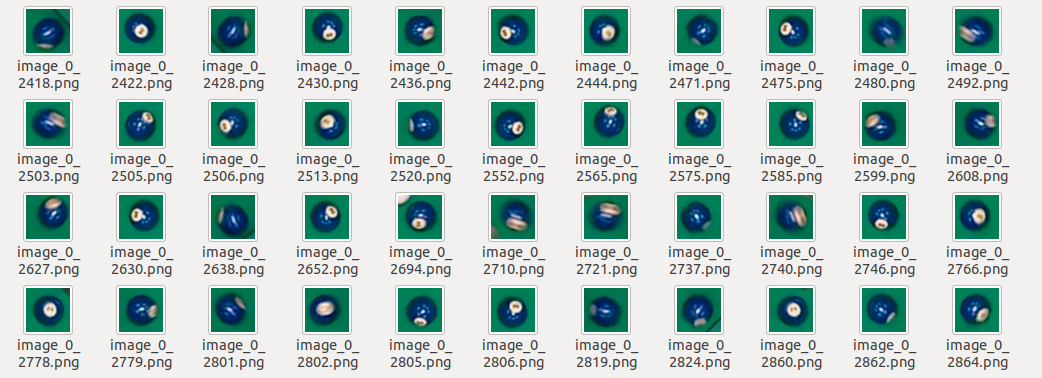
\includegraphics[width=15cm]{./images/obrazki/klasyfikacja/augmented_data.png}
       \caption{Fragment utworzonego datasetu.}
       \label{dataset}
    \end{figure}

    
    Wykryte i sklasyfikowane bile, co przedstawia rysunek \ref{bp_classified}, wysyłane są do końcowego procesu – \textbf{OutputModule}. Wartości wszystkich punktów normalizowane są do przestrzeni, gdzie prawy dolny punkt stołu ma współrzędne $(2, 1)$. Pozwala to uniezależnić wyświetlanie danych od rozmiaru klatki wejściowej. Parametry progowania, minimalny oraz maksymalny promień wykrywania bil, oraz wszystkie parametry metody \textbf{HoughCircles} konfigurowalne są z poziomu interfejsu aplikacji, co pozwala na dynamiczne ich dostosowywanie.

    \begin{figure}[!htb]
        \centering
        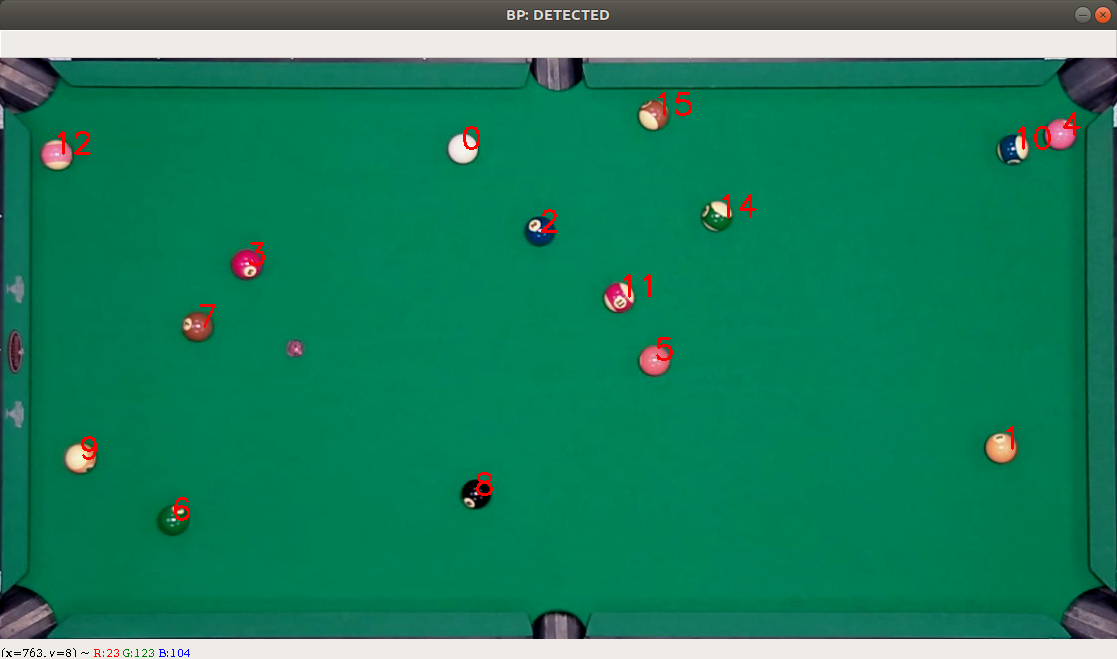
\includegraphics[width=15cm]{./images/obrazki/klasyfikacja/bp_classified.png}
        \caption{Ostateczny produkt uzyskiwany w \textbf{BallProcesor} - wykryte i sklasyfikowane bile.}
        \label{bp_classified}
    \end{figure}

\subsection{Kij}

Uzyskiwanie sprogowanego obrazu odbywa się podobnie jak w przypadku detekcji bil, ale przy innych, bardziej odpowiednich dla tego problemu, parametrów, które tak jak w przypadku detekcji bil konfigurowalne są z poziomu interfejsu użytkownika. Uzyskany obraz sprogowany przedstawiony został na rysunku \ref{cp_thresh}

\begin{figure}[!htb]
    \centering
    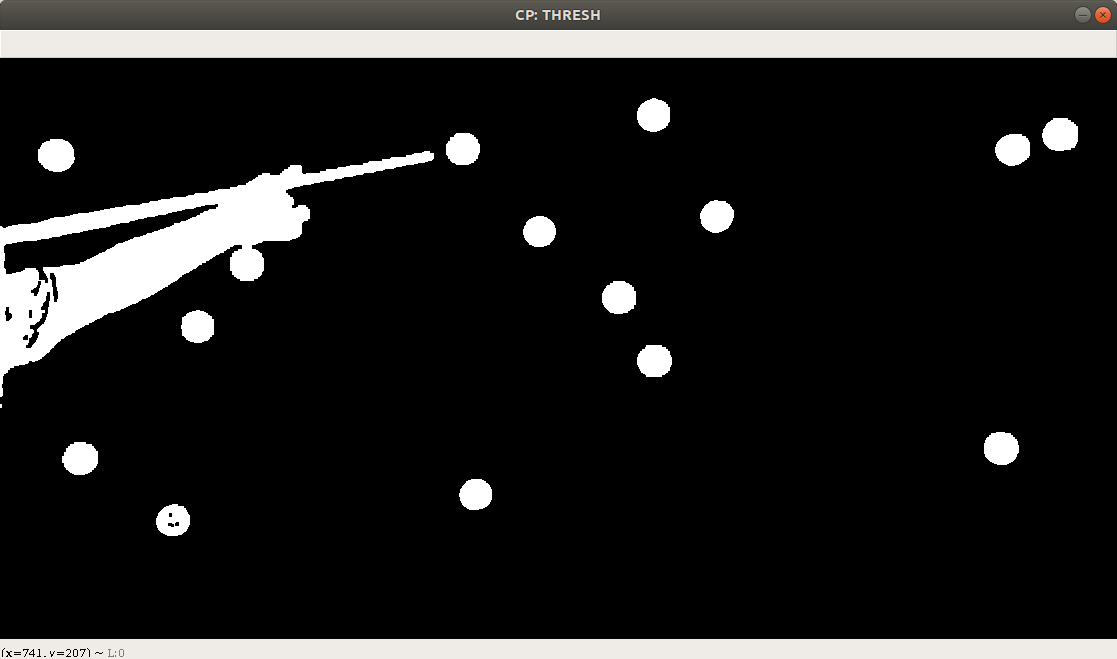
\includegraphics[width=15cm]{./images/obrazki/cp/cp_thresh.png}
    \caption{Sprogowany obraz po przeprowadzeniu operacji morfologicznych dla \textbf{CueProcessor}.}
    \label{cp_thresh}
\end{figure}

\newpage

Do detekcji kijów wykorzystano metodę \textbf{HoughLinesP} opisaną na stronie \cite{HoughLinesP}, która wykorzystuje probabilistyczny algorytm transformacji Hougha \cite{ProbabilisticHoughTransform}. Pozwala ona na uzyskanie współrzędnych początków i końców kijów, które wysyłane są do \textbf{OutputModule}. Podobnie jak w przypadku \textbf{BallProcessor}, przed wysłaniem, współrzędne początków i końców kijów normalizowane są do przestrzeni, gdzie prawy dolny punkt stołu ma współrzędne $(2, 1)$

\begin{figure}[!htb]
    \centering
    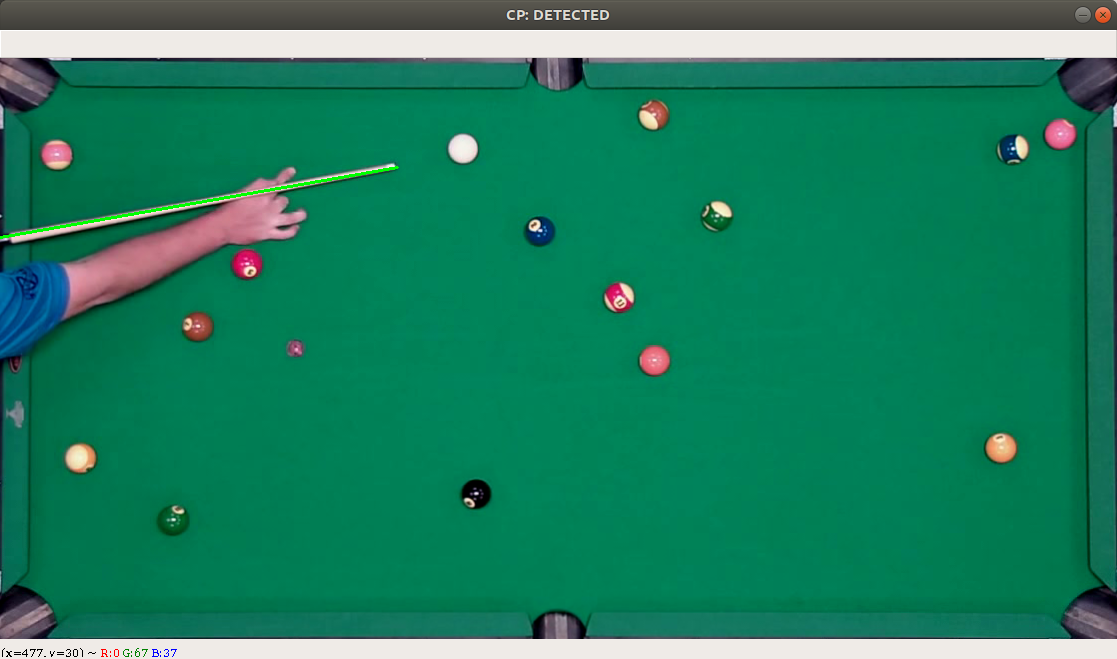
\includegraphics[width=15cm]{./images/obrazki/cp/cue_detected.png}
    \caption{Wykryty kij.}
    \label{cue_detected}
\end{figure}



\section{Interfejs użytkownika}

Wyświetlanie stołu odbywa się w komponencie \textbf{PoolVD}. Aplikacja webowa stworzona z wykorzystaniem frameworka Vue i Vuetify, na komponencie Canvas rysuje stół wraz z aktualną, wydedukowaną zawartością łuz (rysunek \ref{pool1}). Rysowanie elementów odbywa się ze wsparciem frameworka KonvaJS\cite{konva}. Białe półprzezroczyste elipsy wokół łuz obrazują obszar działania dedukcji wpadnięcia bili do łuzy. Pełny widok interfejsu graficznego przedstawia rysunek~\ref{interface}.

\begin{figure}[!htb]
    \centering
    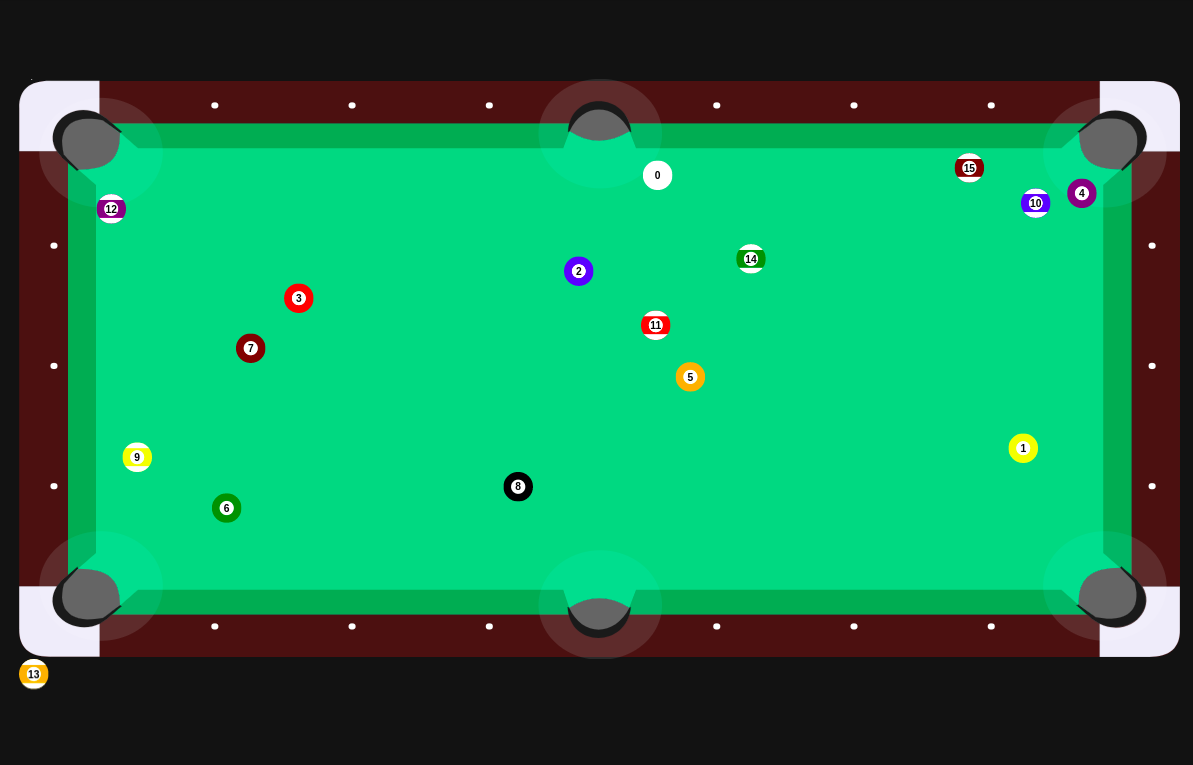
\includegraphics[width=15cm]{./images/pool1.png}
    \caption{Widok stołu w komponencie \textbf{PoolVD}.}
    \label{pool1}
\end{figure}

Aplikacja posiada wysuwalny panel (rysunek \ref{options}), z którego poziomu można zmieniać parametry detekcji i dedukcji. Zmiany ustawień detekcji generują opisane wcześniej zdarzenia, które odbierane są przez komponent \textbf{VideoProcessor}. Zmiany ustawień dedukcji mają efekt tylko na poziomie komponentu \textbf{PoolVD}.

\begin{figure}[!htb]
    \centering
    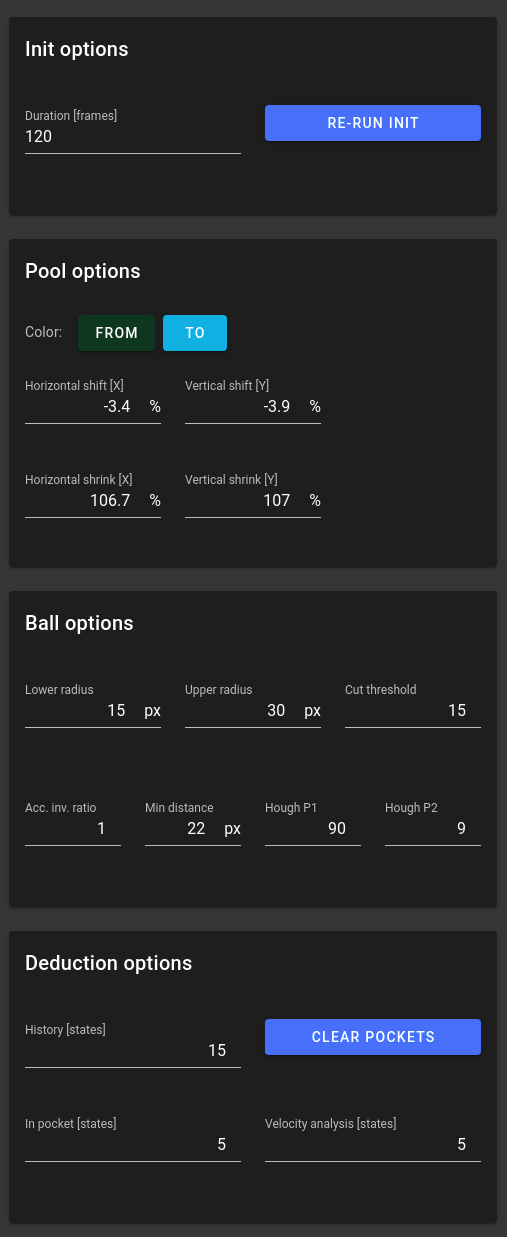
\includegraphics[height=19cm]{./images/options.png}
    \caption{Panel opcji w komponencie \textbf{PoolVD}.}
    \label{options}
\end{figure}

Z racji na możliwość powstania przesunięcia i zaburzeń proporcji stołu w kamerze ustawienia pozwalają na zmianę przesunięcia i skali wyświetlanych elementów stołu. Jest to końcowym etapem bezpośrednio poprzedzającym wyświetlanie elementów stołu, więc dedukcja i analiza pozycji odbywa się na danych otrzymanych od komponentu \textbf{VideoProcessor}.

\begin{figure}[!htb]
    \centering
    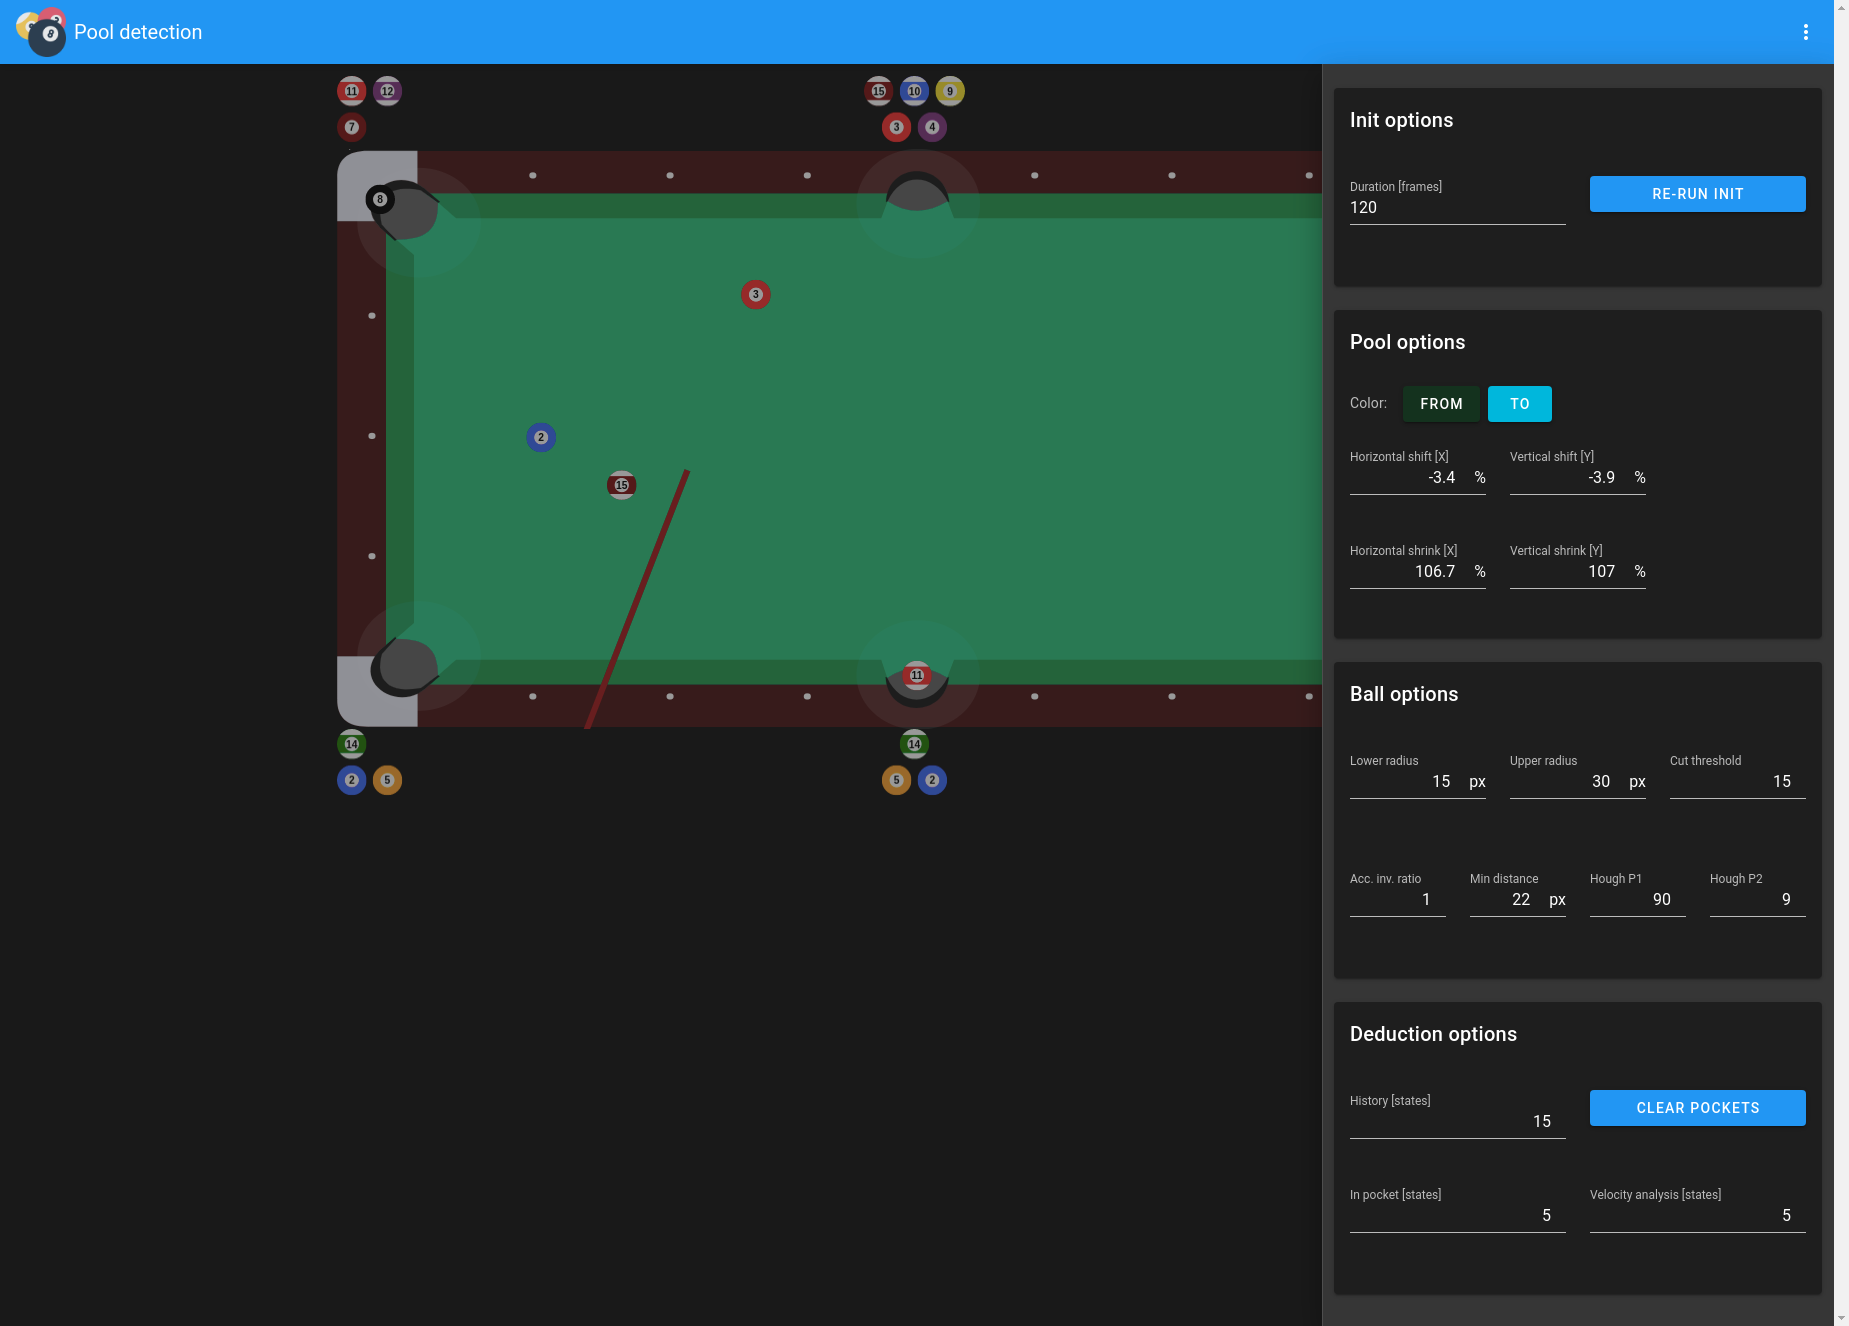
\includegraphics[width=15cm]{./images/interface.png}
    \caption{Interfejs komponentu \textbf{PoolVD} z testowymi danymi.}
    \label{interface}
\end{figure}


\FloatBarrier


\section{Uruchomienia systemu}
W calu uruchomienia systemu należy udostępnić źródło danych i uruchomić dwa główne komponenty - \textbf{VideoProcessor} i \textbf{PoolVD}. Wszystkie polecenia muszą być wykonane z katalogu głównego projektu.

\subsubsection{Źródło danych}
Źródłem danych może być dowolny strumień wideo przesłany z użyciem protokołu UDP. Podczas pracy nad projektem źródłem danych był plik MP4 streamowany z użyciem skryptu za pomocą komendy:
\begin{lstlisting}
$ ./video_processor/test/stream.sh ./video_processor/test/videos/test3.mp4 127.0.0.1:8444
\end{lstlisting}
Powyższa komenda wysyła dane na port 8444 hosta lokalnego wykorzystując narzędzie ffmpeg.

\subsubsection{VideoProcessor}

Komponent \textbf{VideoProcessor} powinien być uruchomiony za pomocą następującej komendy:

\begin{minipage}{\linewidth}

\begin{lstlisting}
$ pipenv install
$ pipenv shell
$ python3 -m video_processor.src.main -p 8444 -c 8888 -w 1280 -ht 720 -f 30
\end{lstlisting}
\end{minipage}

Argumentami komendy są kolejno port źródła danych, port nasłuchu klientów \textbf{PoolVD}, wysokość klatki, szerokość klatki i liczba klatek na sekundę materiału źródłowego. Uruchomienie modułu wymaga wcześniejszego zainstalowania zależności zdefiniowanych w pliku Pipfile narzędziem Pipenv.
\subsubsection{PoolVD}
Uruchomienie komponentu \textbf{PoolVD} odbywa się w oparciu o środowisko NodeJS i narzędzia VueCLI4 \cite{vuecli} z wykorzystaniem wersji deweloperskiej serwera. Port połączania z komponentem \textbf{VideoProcessor} (8888) w obecnej wersji jest na stałe wpisany w kod. Aplikacja dostępna jest pod adresem \lstinline{localhost:8080}.

\begin{minipage}{\linewidth}
\begin{lstlisting}
$ ( cd pool_vd && npm install )
$ ( cd pool_vd && npm run serve )
\end{lstlisting}
\end{minipage}

\section{Podsumowanie}

\subsection{Zrealizowane założenia}

System w obecnej formie realizuje odbieranie materiału źródłowego, jego przetwarzanie i wysyłanie danych do użytkownika. Pozwala na detekcję i klasyfikację bili oraz na detekcję kijów. Aplikacja użytkownika pozwala na modyfikację parametrów klasyfikacji i detekcji oraz odpowiada za dedukcję stanu gry - odrzucanie błędów klasyfikacji i detekcji oraz za wykrywanie wpadnięć bili do łuzy. Parametry dedukcji są również konfigurowalne.

\subsection{Możliwości rozwoju}

Język Python, w którym napisany został komponent \textbf{VideoProcessor} doskonale sprawdza się w prototypowaniu złożonych rozwiązań dotyczących przetwarzania obrazu ze względu na dostępność szerokiego wachlarza bibliotek. Sprawdza się nawet w przypadku systemów działających na wielu rdzeniach procesora, mimo ograniczeń jakie niesie ze sobą GIL\cite{gil}. Niestety skonstruowane przez nas rozwiązanie przesyłania stanów stołu wiązało się z użyciem korutyn, których wykonywanie w połączeniu z wieloprocesorowością i z wykrozystaniem obu kolejek bili i kilów, prowadziło do nieprzewidywalnych zachowań i braku stabilności przesyłania stanu stołu. Dlatego też nie udało się zaimplementować efektywnego przesyłania pozycji kijów. Rozwijając projekt można przebudować moduł \textbf{OutputModule} tak, aby sprawnie obsługiwał protokół WebSocket, który jest podstawą do wydajnego przesyłania danych do aplikacji webowej komponentu \textbf{PoolVD}.

Rozwój projektu może wiązać się oczywiście też z poprawianiem struktury sieci neuronowej oraz zebranych lepszych danych treningowych obejmujących różne stoły i warianty kolorów bili. Wydajność detekcji i klasyfikacji bili ma bardzo duże znaczenie w procesie dedukcji stanu stołu.

\clearpage
\newpage

\printbibliography

\end{document}